%% LyX 2.3.6 created this file.  For more info, see http://www.lyx.org/.
%% Do not edit unless you really know what you are doing.
\documentclass[english]{article}
\usepackage[T1]{fontenc}
\usepackage[latin9]{inputenc}
\usepackage{color}
\usepackage{graphicx}
\usepackage{babel}
\begin{document}
Human activity recognition using deep electroencephalography learning.

introduces a deep learning-based framework for classifying EEG artifacts
(FCEA)

involving a Convolutional Neural Network and a Long Short-Term Memory
Recurrent Neural Network.

a 3-class dataset of EEG activities was created.

ameras, accelerometers, gyroscopes and sound sensors have been used
to detect the movement of users in automatic Human Activity Recognition
(HAR) systems.

In HAR system design, Machine Learning (ML) algorithms have made significant
progress in the extraction of human activity fea- tures from sensor
data.

7\% of the studies used only a combination of CNNs and RNNs, whereas,
40 \% used only CNNs and 14 \% used only RNNs.

whilst reading printed text, speaking out loudly and watching a TV
program.

The technologies used for detecting human actions are commonly based
on heterogeneous sensors placed throughout the environment, such as
cameras and wearable sensors equipped with accelerometers, gyroscopes
and biosensors {[}1--4{]}. Cameras provide video data in form of
a 3D matrix.

The CNNs are more appropriate for learning and interpreting camera
and motion-detection sensor data. The LSTM networks are not capable
of classifying video data alone. They, however, attain a desirable
classification performance when they are used for modeling accelerometer
and gyroscope raw data, as well as the feature maps populated by a
CNN {[}2{]}.

Moreover, the smartphone and smartwatches which have been mostly used
in HAR, are not suitable for recognizing facial activities.

Analyzing and training a neural network on EGG (Electroencephalography)
data involves several steps. Here's a general guide to get you started:

1. {*}{*}Understand the EGG Data:{*}{*} - Familiarize yourself with
the structure and characteristics of the EEG data you have. Understand
the number of channels, sampling frequency, and the duration of the
recordings.

2. {*}{*}Preprocess the Data:{*}{*} - Clean the data by removing artifacts
and noise. Common preprocessing steps include filtering, artifact
removal, and normalization. - Segment the data into epochs. This involves
dividing the continuous EEG signal into smaller, manageable chunks,
often aligned with specific events or stimuli.

3. {*}{*}Feature Extraction:{*}{*} - Extract relevant features from
the EEG epochs. Common features include power spectral density, time-domain
features, and statistical measures.

4. {*}{*}Data Splitting:{*}{*} - Split your data into training, validation,
and test sets. This is crucial for evaluating your model's performance
on unseen data.

5. {*}{*}Build a Neural Network Model:{*}{*} - Choose or design a
neural network architecture suitable for your task. For time-series
data like EEG, recurrent neural networks (RNNs) or long short-term
memory networks (LSTMs) are often used. Alternatively, you can use
1D convolutional neural networks (CNNs).

6. {*}{*}Model Training:{*}{*} - Train your neural network on the
training dataset. Use the validation set to monitor the model's performance
and prevent overfitting. - Experiment with different hyperparameters,
architectures, and regularization techniques to improve performance.

7. {*}{*}Evaluation:{*}{*} - Evaluate your trained model on the test
set to assess its generalization to new, unseen data. - Use appropriate
metrics for your task, such as accuracy, precision, recall, or specific
metrics relevant to EEG analysis.

8. {*}{*}Interpretation:{*}{*} - Interpret the results and gain insights
into the neural network's performance. Understand which features contribute
most to the model's predictions.

9. {*}{*}Fine-Tuning and Optimization:{*}{*} - If necessary, fine-tune
your model or explore advanced techniques to improve performance,
such as transfer learning or ensemble methods.

10. {*}{*}Documentation and Reporting:{*}{*} - Document your approach,
findings, and any challenges faced during the analysis. This is crucial
for reproducibility and collaboration.

Remember that the specific steps and techniques may vary based on
the nature of your EEG data and the task you are trying to solve.
Always adapt your approach based on the characteristics of your data
and the goals of your analysis.

\textcolor{blue}{Paper: A Tutorial on Human Activity Recognition Using
Body-Worn Inertial Sensors }

Reference: (ANDREAS BULLING, Max Planck Institute for Informatics,
Germany ULF BLANKE, Swiss Federal Institute of Technology (ETH) Zurich,
Switzerland BERNT SCHIELE, Max Planck Institute for Informatics, Germany).

while recognizing the task of brushing one's teeth.

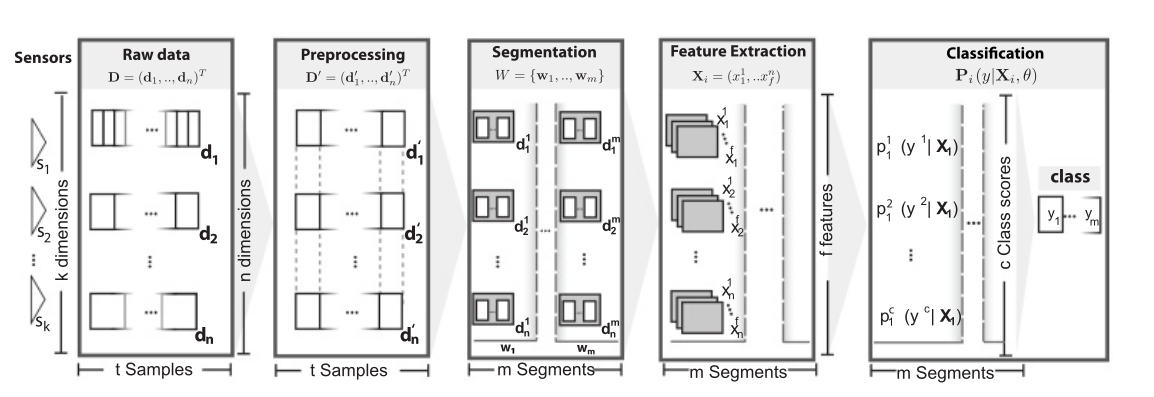
\includegraphics[scale=0.25]{ActivityRecognitionChain}

~~\\
\\

Raw signals ($D$) are first processed ($D'$) and split into $m$ segments ($W_i$) from which feature vectors ($X_i$) are extracted. Given features ($X_i$), a model with parameters $\theta$ scores $c$ activity classes $Y_i = \{y^1, \ldots, y^c\}$ with a confidence vector $p_i$. 
\end{document}
